\chapter{Telematik}

Zusammenfassung der Vorlesung "`Telematik"' aus dem Wintersemester 2016.\footnote{\url{https://telematics.tm.kit.edu/ws201617_telematik.php}}

\section{Transportprotokolle}

\subsection{Grundlegende Komponenten}

\subsubsection{TCP-Grundlagen}
\begin{itemize}
	\item \textbf{TCP-Verbindungsverwaltung}
	\begin{itemize}
		\item Identifikation einer TCP-Verbindung: Quell-/Zieladresse sowie Quell-/Zielport
		\item Verbindungsaufbau: Server wartet, Client initiiert Verbindung
		\item 3-Wege-Handshake
		\begin{enumerate}
			\item Client \(\rightarrow\) Server: \texttt{TConReq(SYN=1,seq=client\_isn)}
			\item Client \(\leftarrow\) Server: \texttt{TConCnf(SYN=1,ACK=1,seq=server\_isn,ack=client\_isn+1)}
			\item Client \(\rightarrow\) Server: \texttt{ACK(SYN=0,ACK=1,seq=client\_isn+1,ack=server\_isn+1)}
		\end{enumerate}
		\item Zusätzlich: Festlegen der initialen Sequenznummer (\texttt{isn}), Bekanntgabe der Größe des Flusskontrollfensters, Allokation der Puffer
		\item Format einer TCP-Dateneinheit\footnote{\url{https://upload.wikimedia.org/wikipedia/de/f/fd/TCP_Header.svg}}\\
			\begin{minipage}{\linewidth}
				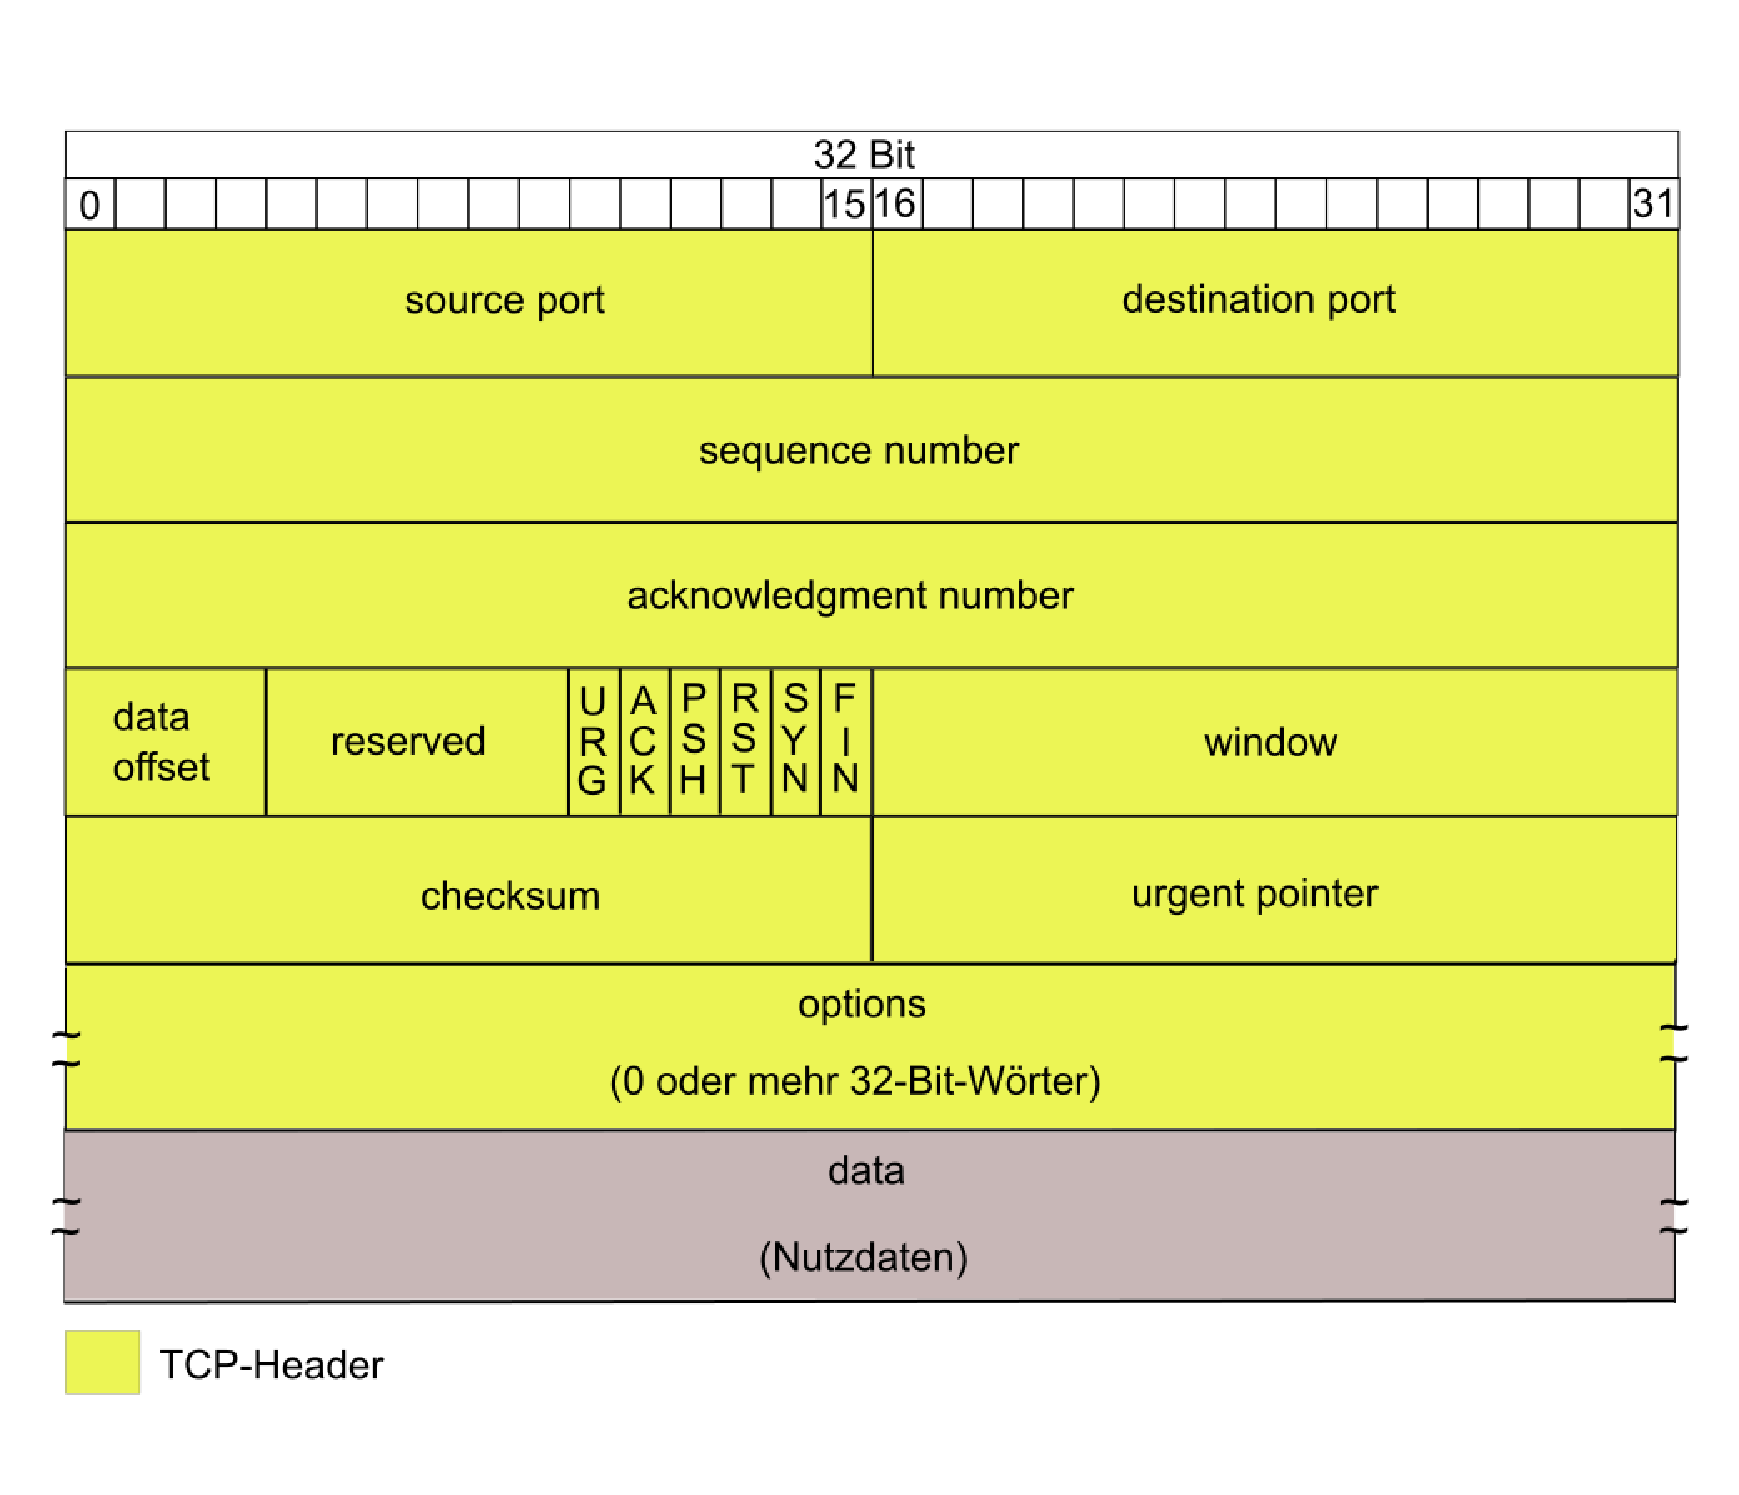
\includegraphics[scale=0.38]{telematik/TCP_Header.pdf}
			\end{minipage}
	\end{itemize}
	\item \textbf{Flusskontrolle zur Schutz des Empfängers vor zu hoher Last}
	\begin{itemize}
		\item Dynamische Anpassung des Empfangsfenster auf Empfängerseite, um die aktuelle verfügbare Puffergröße mitzuteilen. \texttt{RcvWindow} bezeichnet den Anteil des \texttt{RecvBuffer}, das frei ist (jeweils absolute Werte)
		\item Problem: Empfänger meldet ein volles Empfangsfenster. Woher weis der Sender, ab wann er wieder senden darf? \(\rightarrow\) Empfänger muss auch bei vollem Empfangsfenster Dateneinheiten mit einem Byte Länge quittieren (\textit{Zero Window Probing})
	\end{itemize}
	\item \textbf{Angriffe auf den Verbindungsaufbau: SYN-Flooding}
	\begin{itemize}
		\item Massenhaftes Senden von SYN-Dateneinheiten ohne Verbindungsaufbau. Problem: Zustandshaltung auf Empfängerseite für halboffene Verbindungen. Folge: Ressourcen erschöpft, Empfänger kann keine Dateneinheiten mehr annehmen
		\item Lösung: SYN-Cookies
		\begin{itemize}
			\item Verhinderung der Zustandshaltung bis zum letztmöglichen Zeitpunkt: Beginn der Zustandhaltung erst bei Empfang des \texttt{ACK}
			\item Realisierung: Ermittlung der Zustandsinformationen auf Empfängerseite anhand der Informationen aus \texttt{ACK(SYN=0,ACK=1,seq=client\_isn+1,ack=server\_isn+1)}
			\item Kodierungsbeispiel: Zeitstempel zur Verhinderung von Replay-Attacken (5 Bit); ausgewählte MSS aus acht vordefinierten Werten (3 Bit); Hash über Quelladresse und -port sowie Zieladresse und -port, verifiziert dass der Client bereits \texttt{SYN} durchgeführt hat /24 Bit). Daraus entsteht die 32 Bit initiale Sequenznummer des Servers
			\item Nachteil: Vergleichsweise kurze Sequenznummer (32 Bit) reicht nicht für zusätzliche TCP-Optionen und limitiert MSS-Größen auf vordefinierte Werte
			\item Idee: Cookie erst einsetzen, wenn nötig (volle Warteschlange oder Ressourcenengpass)
		\end{itemize}
	\end{itemize}
\end{itemize}

\subsubsection{Staukontrolle}
\begin{itemize}
	\item Beobachtung: Unverhältnismäßiger Leistungseinbruch an Engstellen bei großem Datenaufkommen zwischen zwei schnelleren Netzen \(\rightarrow\) Warteschlangenmanagement notwendig
	\item \textbf{Einfaches Warteschlangenmanagement}
	\begin{itemize}
		\item Puffer im Router voll, nächste Dateneinheit muss verworfen werden ("`Tail Drop"')
		\item Retransmissiontimer im Client steuert Sendewiederholungen
		\item Problem: Synchronisation. Dateineinheiten von mehreren Verbindungen werden quasi gleichzeitig verworfen
	\end{itemize}
	\item \textbf{Aktives Warteschlangenmanagement}
	\begin{itemize}
		\item Das Netz gibt einen Hinweis auf eine entstehende Stausituation, bevor eine Überlast entsteht
		\item Router verwirft (randomisiert) Dateneinheiten, bevor die Warteschlange voll ist. Sorgt für Fairness und verhindert globale Synchronisation
		\item Verfahren
		\begin{itemize}
			\item Konkrete Implementierung: Random Early Detection (RED)
			\begin{itemize}
				\item Wahrscheinlichkeit, dass eine Dateneinheit verworfen wird, steigt linear mit der Warteschlangenlänge
			\end{itemize}
		\end{itemize}
	\end{itemize}
	\item \textbf{Self-Clocking}
	\begin{itemize}
		\item Szenario: Verbindung zweier Netze über langsames Weitverkehrsnetz. Dateneinheiten benötigen bei der langsamen Übertragung mehr Zeit als in den lokalen Netzen. Dadurch kommen sie verzögert beim Empfänger an, welcher sie entsprechend "`langsam"' quittiert. Durch den entstehenden Takt weis der Sender, wie schnell er senden kann. Aber: Wie soll die "`Uhr"' gestartet werden?
		\item Wieso wird kein Gleichgewicht erreicht?
		\begin{itemize}
			\item Verbindung kommt nicht ins Gleichgewicht. Mögliche Auslöser: Neue Verbindung/Neustart, automatische Anpassung der Datenrate und Verzögerung
			\item Sender sendet neue Dateneinheiten zu früh
			\item Ressourcenbeschränkungen verhindern Gleichgewicht
		\end{itemize}
		\item Slow-Start (Einzelverbindung)
		\begin{itemize}
			\item Erhöhung der Anzahl der gesendeten Dateneinheiten über die Zeit durch Einführung eines Staukontrollfensters (\texttt{Staukontrollfenster < Flusskontrollfenster}). Verhindert burstartiges Senden der Quelle, was zu vielen Sendewiederholungen führen würde
			\item Bei Verbindungsstart oder Verlust einer Dateneinheit wird das Staukontrollfenster zurückgesetzt
			\item Startverhalten ohne Slow-Start: Viele Sendewiederholungen durch Paketverluste. "`lineares Zickzackwachstum"', das weit hinter der verfügbaren Datenrate zurück bleibt (effektive Nutzung bei 35\%)
			\item Startverhalten mit 2s Slow-Start: Keine Sendewiederholungen, Datenrate nahezu am verfügbaren Maximum. Effiziens abhängig von Vebrindungsdauer, da dann die langsame Slow-Start-Phase an Gewicht verliert
		\end{itemize}
		\item Congestion Avoidence (Simultane, konkurrierende Verbindungen)
		\begin{itemize}
			\item Ohne Congestion Avoidance: Sehr viele Sendewiederholungen (nahezu 50\% im Experiment), sehr unfaire Aufteilung
			\item Mit Congestion Avoidance: Sehr wenige Sendewiederholungen, verschiedene Quittungsstrategien möglich
			\item Zusammenfassung: Faire Aufteilung der verfügbaren Kapazität, langsames Herantasten durch lineares Erhöhen des Staukontrollfensters sowie kaum Sendewiederholungen
		\end{itemize}
		\item Fast Retransmit
		\begin{itemize}
			\item Beobachtung: Nicht jede nicht in Reihenfolge erhaltene Dateneinheit ist ein Indiz für eine Überlastung des Netzes
			\item Mechanismus zur Staukontrolle: Sendewiederholung beim Empfangeiner definierten Anzahl duplizierter Quittungen
			\item Vorgehen: Warten auf Timerablauf, dann Sendewiederholung (Wartezeit größer Umlaufzeit \texttt{RTT})
		\end{itemize}
	\end{itemize}
	\item \textbf{Staukontrolle}
	\begin{itemize}
		\item Implizite Staukontrolle: Implizite "`Anzeige"' einer Stausituation ohne explizite Unterstützung des Netzes
		\begin{enumerate}
			\item TCP-Tahoe
			\begin{itemize}
				\item Mechanismen: Slow Start, Timeout, Congestion Avoidance, Fast Retransmit
				\item Nach Timeout oder Empfang duplizirter Quittungen: Beginn von Slow Start
				\item Grundlegende Vorgehensweise: Additives Erhöhen des Congestion Window \texttt{CWnd}, multiplikatives Erniedrigen (\texttt{AIMD})
			\end{itemize}
			\item TCP-Reno
			\begin{itemize}
				\item Zusätzlich zu TCP-Tahoe: Fast Recovery (siehe unten)
				\item Unterscheidet zwischen \textit{schweren Stausituationen} (Timeout bei Ausstehenden Quittungen) und \textit{leichten Stausituationen} (Empfang von duplizierten Quittungen)
				\item Leichte Stausituationen: Kein Rücksetzen auf Slow Start, da Quittungsempfang impliziert, dass weiter neue Daten empfangen worden sind
				\item Schwere Stausituationen: Rücksetzen auf Slow Start wie bei TCP-Tahoe
				\item Fast Recovery
				\begin{itemize}
					\item Szenario: Empfang einer festgelegten Anzahl Quittungen (beispielsweise drei)
					\item Idee: Senden neuer Dateneinheiten, auch wenn der Fehler noch nicht behoben ist (Self-Clocking geht weiter)
					\item Vorgehen: Reduzierung der Belastung (halbieren des Staukontrollfensters) sowie Fast Retransmit
				\end{itemize}
			\end{itemize}
		\end{enumerate}
		\item Explizit Congestion Notification (ECN): Explizite Staukontrolle mit Netzunterstützung
		\begin{itemize}
			\item Idee: Erkennen von Stausituationen im Netz über den Füllstand der Warteschlange (setzt aktives Warteschlangenmanagement voraus) sowie markieren der IP-Einheiten vor Weiterleitung zum Empfänger. Dieser informiert den Sender, um das Staukontrollfenster zu regeln
			\item Signalisierung in Schicht 3 (IP): Nutzung zweier Bits im TOS-Feld der Dateneinheit
			\item Signailisierung in Schicht 4 (TCP): Einführung zusätzlicher Flags im TCP-Kopf
			\begin{itemize}
				\item \texttt{ECE}-Bit: Signalisiert dem Sender die Stausituation (Sender \(\leftarrow)\) Empfänger)
				\item \texttt{CWR}-Bit: Bestätigt dem Empfänger den Erhalt einer Staumeldung (Sender \(rightarrow\) Empfänger)
			\end{itemize}
		\end{itemize}
	\end{itemize}
\end{itemize}

\subsubsection{Fairness}
\begin{itemize}
	\item TCP-Verbindungen konkurrieren um Ressourcen des Netzes \(rightarrow\) faire Aufteilung angestrebt
	\item \textbf{Probleme}
	\begin{itemize}
		\item "`Gierige Nutzer"': Faire Verteilung bezieht sich auf TCP-Verbindungen. Kann daher mehrere Verbindungen gleichzeitig öffnen. Gegenmaßnahme: Verteilung der Kapazität pro Benutzer
		\item "`Gieriger Empfänger"': Da Quittungsverhalten der Empfängerinstanz die Ressourcenzuteilung beeinflusst, kann dieser mehr oder scheller Quittungen senden. Das Staukontrollfenster öffnet sich schneller, damit erhält die Verbindung mehr Ressourcen
		\begin{enumerate}
			\item Mehrere Quittungen pro empfangener Dateneinheit: Sequenznummern zählen Bytes, Staukontrollfenster zählen Dateneinheiten. Bestätigt der Empfänger jede Dateneinheit in mehreren "`Häppchen"', so öffnet sich das Staukontrollfenster schneller
			\item Quittungen schneller senden als Daten empfangen werden. Protokolländerung notwendig
			\item Identische Quittungen mehrfach senden: Fehlende Dateneinheit wird erneut gesendet. Bei TCP-Reno läuft Self-Clocking weiter \(\rightarrow\) Staukontrollfenster wird weiter geöffnet
		\end{enumerate}
	\end{itemize}
\end{itemize}

\subsection{Analyse und Randbedingungen}

\subsubsection{Analyse von TCP: Modelle}
\begin{itemize}
	\item Analytische Beurteilung hinsichtlich Durchsatz und Latenz
	\item Zentrale Fragen: Ist \texttt{TCP} für meine Zwecke geeignet?`Welche Leistung kann ich erwarten?
	\item \texttt{Periodisches Modell}
	\begin{itemize}
		\item Vereinfachte Betrachtung des langfristigen Verhaltens ohne Slow-Start und Sendewiederholungen \(\rightarrow\) Staukontrollfenster bildet "`perfekte"' Sägezahnkurve mit periodischen Paketverlusten
		\item Vorgehen: Berechne die Anzahl übertragender Dateneinheiten \(Y_i\) zwischen zwei aufeinenader folgenden Verlusten von Dateneinheiten (also in einem Durchlauf)
		\item Durchschnittliche Übertragungsrate: \(X=\frac{1}{RTT}\cdot\sqrt{\frac{3}{2p}} = 1,22 \cdot \frac{1}{RTT\cdot\sqrt{p}}\)
		% TODO: mehr?
	\end{itemize}
	\item \texttt{Detaillierstes Verlust-Modell}
	\begin{itemize}
		\item Unterschied zum periodischen Modell: Verluste nicht mehr periodisch \(\rightarrow\) Dauer der Durchläufe nicht mehr gleich lang
		% TODO: mehr?
	\end{itemize}
\end{itemize}

\subsubsection{Hohe Datenraten}

\subsubsection{Kurze Latenzen}
\begin{itemize}
	\item \textbf{TCP und Web}
	\begin{itemize}
		\item Interaktiver Dienst, Besucher äußerst ungeduldig \(\rightarrow\) Antwortzeit entscheident
		\item Verwendung von \texttt{HTTP} in \texttt{TCP} \(\rightarrow\) bei jedem Klick wird mindestens eine \texttt{TCP}-Verbindung aufgebaut \(\rightarrow\) sehr viele Verbindungsaufbauten für wenig Übertragung
		\item Bei kleinen Objekten dominieren RTTs die Antwortzeit; Slow-Start hat entscheidenden Einfluss auf die Verzögerung
		\item Möglichkeiten zur Verbesserung
		\begin{itemize}
			\item Größeres initiales Staukontrollfenster: Mindestens 10 \texttt{TCP}-Segmente mit \(\sim 15\) KByte, da 90\% aller Web-Objekte \(\le 16\) KByte sind
		\end{itemize}
	\end{itemize}
	\item \textbf{TCP und Web}
	\begin{itemize}
		\item
	\end{itemize}
\end{itemize}


\subsection{Aktuelle Entwicklungen}



\section{Routing im Internet}

\subsection{Grundlagen}
\begin{itemize}
	\item Aufgaben: Weiterleitung sowie Kopplung von Netzen \(\rightarrow\) Verknüpfung einzelner Übertragungsabschnitte zu einer E2E-Übertragung
	\item Wegfindung im Kommunikationssystem: Weiterleitung im Router anhand Weiterleitungstabelle. Schnelle Weiterleitung mittels kurzen Warteschlangen und kleinen Tabellen
	\begin{itemize}
		\item Pro Dateneinheit ein Lookup in Weiterleitungstabelle
		\item \textit{Metriken} (üblicherweise Ganzzahl) zur Bewertung von Übertragungsabschnitten
		\item \textit{Policies} als Betreibervorgabe zur Routingstrategie. Bsp.: Bevorzugt bestimmten Nachbarn wählen
	\end{itemize}
	\item Herausforderung: Weiterleitung in Line-Speed. Dazu extrem teure, spezielle Cisco Hardware mit bis zu \texttt{1,2 Tbit/s} pro Chassi \(\rightarrow\) nur wenige dutzend Nanosekunden Bearbeitungszeit pro Dateneinheit
	\item Das Internet Protokoll (IP): Unzuverlässiger Dienst; keine Kontexthaltung in Zwischensystemen; keine Verbindungen
\end{itemize}

\subsubsection{Router}
\begin{itemize}
	\item \textbf{Weiterleitung}
	\begin{itemize}
		\item Aufbau Weiterleitungstabelle: \(Prefix \rightarrow Port\) mit Default-Regel am Ende (falls keine der oberen Regeln zutrifft)
		\item Falls mehrere Einträge passen: \textit{Longest Prefix Matching}
		\item Suche in Line-Speed: Verfahren
		\begin{itemize}
			\item Binärer Trie: Pfadabstieg entsprechend den Adressbits
			\item Patricia Trie zur kombrimierten Speicherung von Binärbäumen: Knoten ohne Verzweigung überspringen und dabei Index vom nächsten relevanten Bit merken
			\item Problem bei Bäumen: Eintrag im Worst-Case erst nach \(N=Adress\_Laenge\) Schritten gefunden
			\item Hash-Tabelle zur Beschleunigung des Lookups
			\begin{itemize}
				\item Longest-Prefix nicht praktikabel \(\rightarrow\) Suche nach der kompletten Adresse
				\item Trie-Lookups lediglich, wenn kein Eintrag in der Hashtabelle vorhanden ist
			\end{itemize}
			\item Hardwarerealisierung \textit{Content-Addressable Memory} (CAM)
			\begin{itemize}
				\item Speicherzugriff über einen Teil des gespeicherten Inhalts
				\item Sehr schnell, da in Hardware realisiert; paralleler Zugriff möglich
				\item Anwendung hier: Abbildung \(IPAdresse \rightarrow Ausgangsport\)
				\item Problem: Zuordnung einzlner Adressen wenig hilfreich. Daher \textit{Ternary Content-Addressable Memory} mit dont-care Bits \(\rightarrow\) Suche nach Präfixen möglich
			\end{itemize}
		\end{itemize}
		\item Aufgaben bei Weiterleitung: Header überprüfen; TTL aktualisieren; Prüfsumme neu berechnen; Lookup; Fragmentierung; Behandlung von IP-Optionen; ggf. Klassifizierung und Priorisierung
		\item Generische Router-Architektur: Der Routingprozessor behandelt lediglich die Kontrolldateneinheiten. Alle Komponenten außer der Routingprozessor puffern. Zielkonflikt Leistungsfähigkeit vs. Kosten\\\\
		\begin{figure}[!h]
		\centering
		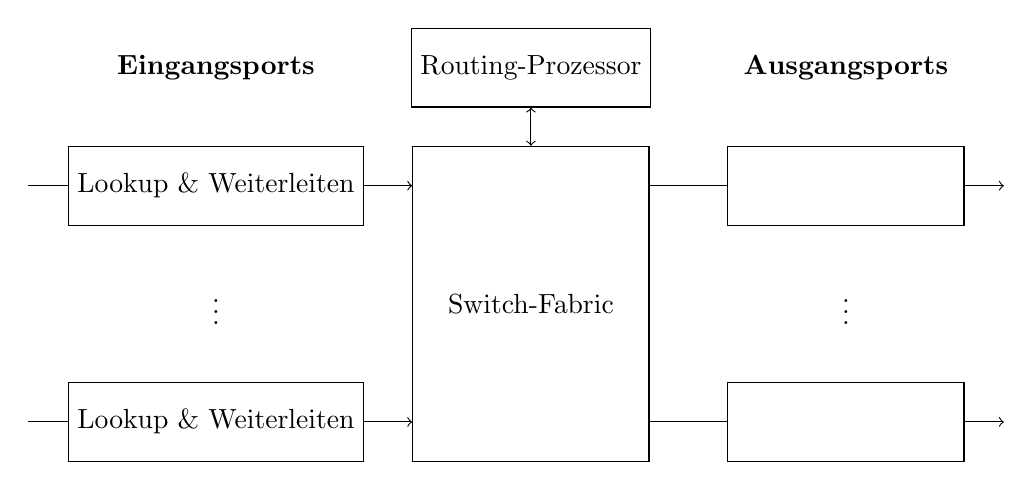
\begin{tikzpicture}
			\node at (4, -3)    [rectangle,draw,minimum height=4cm,minimum width=3cm] (sf)  {Switch-Fabric};
			\node at (4,  0)    [rectangle,draw,minimum height=1cm,minimum width=3cm] (rp)  {Routing-Prozessor};
			\node at (0, -1.5)  [rectangle,draw,minimum height=1cm,minimum width=3cm] (e1)  {Lookup \& Weiterleiten};
			\node at (0, -4.5)  [rectangle,draw,minimum height=1cm,minimum width=3cm] (en)  {Lookup \& Weiterleiten};
			\node at (8, -1.5)  [rectangle,draw,minimum height=1cm,minimum width=3cm] (a1)  {};
			\node at (8, -4.5)  [rectangle,draw,minimum height=1cm,minimum width=3cm] (an)  {};

			\node at (0, 0) {\textbf{Eingangsports}}; \node at (8, 0) {\textbf{Ausgangsports}};
			\node at (0, -3) {\(\vdots\)}; \node at (8, -3) {\(\vdots\)};

			\draw[<->] (sf) edge node {} (rp);
			\draw[-] (e1.west) -- ++(-0.5cm,0) |- (e1); \draw[->] (e1) edge node {} (e1-|sf.west);
			\draw[-] (en.west) -- ++(-0.5cm,0) |- (en); \draw[->] (en) edge node {} (en-|sf.west);
			\draw[-] (sf.east|-a1) edge node {} (a1);   \draw[->] (a1) -| (a1.east) -- ++(0.5cm,0);
			\draw[-] (sf.east|-an) edge node {} (an);   \draw[->] (an) -| (an.east) -- ++(0.5cm,0);
		\end{tikzpicture}
		\end{figure}
	\end{itemize}
	\item \textbf{Switch-Fabric}
	\begin{itemize}
		\item Blockierungen: Gegenmaßnahmen
		\begin{itemize}
			\item \textit{Overprovisioning}: Interne Verbindungen schneller als Eingangsports
			\item Pufferung an den Netzwerkschnittstellen und in Switch-Fabric
			\begin{itemize}
				\item Annahmen zur Vereinfachung: Gleiche Datenrate an allen Ports; alle Pakete gleich groß
				\item Eingangspuffer: Konfliktauflösung am Eingang; geeignete Scheduling-Strategie
				\item Ausgangspuffer: Konfliktauflösung am Ausgang, allerdings \(N\)-fache Vermittlungsgeschwindigkeit der Eingangsports notwendig. Kurze Eingangspuffer zur Aufnahme von jeweils einer Dateneinheit trotzdem notwendig
				\item Verteilter Puffer pro Knotenpunkt in Switch-Fabric: Höherer Speicherbedarf
				\item Zentraler Puffer zur Konflikauflösung: Geringerer Speicher als bei den anderen Puffern nötig, allerfings höhere Anforderungen an die Speicherzugriffszeit 
			\end{itemize}
			\item Backpressur: Überlastsignalisierung an den Eingangsports \(\rightarrow\) Eingangsports reduzieren Last
			\item Parallele Switch-Fabrics
		\end{itemize}
		\item Struktur der Switch-Fabric
		\begin{itemize}
			\item Gemeinsamer Speicher
			\item Bus-/Ringstruktur: Konfliktfreier Zugriff durch Zeitmultiplex; \(Uebertragungskapazitaet \ge \sum Kapazitaet-Eingangsport_i\); Multicast und Broadcast trivial; Anzahl der Anschlüsse sehr begrenzt (\(\le 16\)); Bsp.: \texttt{CISCO 7500}
			\item Koppelmatrix: Alle Eingänge mit alles Ausgängen verbunden; teilweise parallel nutzbar; hoher Verdrahtungsaufwand; unflexibel; besonders effizient bei gleichgroßen Dateneinheiten
			\item Mehrstufige Verbindungsnetzwerke: Ebenfalls alle Eingänge mit allen Ausgängen durch hierarchische Schaltelemente verbunden; geringerer Verdrahtungsaufwand als Koppelmatrix; nicht alle Verbindungen gleichzeitig möglich
		\end{itemize}
	\end{itemize}
\end{itemize}

\subsubsection{Routing-Algorithmen}
\begin{itemize}
	\item Kontrollpfad: Austausch von Routingnachrichten zur Berechnung von Wegen; Routingprotokolle
	\item Datenpfad: Weiterleitung von IP-Paketen
	\item Routingtabelle: \(Prefix \rightarrow Next~Hop\); wird von den Routingalgorithmen erstellt; auf die Anforderungen von Routingalgorithmen optimiert
	\item Weiterleitungstabelle: \(Prefix \rightarrow Ausgangsport\); auf effizienten Lookup optimiert
	\item \textbf{Verteiltes Adaptives Routing}
	\begin{itemize}
		\item Router reagieren denzentral auf sich ändernde Netzsituation (Laständerungen, Linkfehler, etc.)
		\item Adaptiv: Verteiltes Routing mit Informationsaustausch zwischen den Routern
		\item Benötigte Komponenten: Monitoring, Informationsaustausch, Berechnung aktueller/alternativer Routen
	\end{itemize}
	\item \textbf{Distanzvektor vs. Link-State}
	\begin{itemize}
		\item Distanzvektor-Algorithmus: Iterative Berechnung der kürzesten Pfade (beispielsweise via Bellman-Ford-Algorithmus). Umsetzung als \textit{Router Information Protocol} (RIP) im Internet. Routinginformationen werden auf Basis der Informationen von den Nachbarn berechnet und ausgetauscht
		\item Link-State-Algorithmus: Globale Sicht zur Berechnung der kürzesten (Dijkstra-Algorithmus) \(\rightarrow\) jeder Router muss alle Links im Netz kennen \(\rightarrow\) Informationen über lokale Links eines Routers breiten sich im gesamten Netz aus; jeder ROuter berechnet kürzeste Wege selbstständig (replizierte Berechnung)
	\end{itemize}
\end{itemize}

\subsubsection{Routing-Architektur}
\begin{itemize}
	\item Strukturierung in \textit{Autonome Systeme} mit externem (\texttt{Exterior Gateway Protocol}) und internem (\texttt{Interior Gateway Protocol}) Routing \(\rightarrow\) Skalierbarkeit durch zwei logische Ebenen
	\item Autonome Systeme: Erscheinen nach außen als Einheit mit einheitlichem internen Routingprotokoll und gleicherer internen Routingpolicy. IANA delegiert die Zeitteilung
	\begin{itemize}
		\item Aufteilung nach Funktion: Stub-AS (kleines Unternehmen mit einem Provider); Multihomed AS (große Unternehmen mit mehreren Providern); Transit AS (Provider)
		\item Aufteilung nach Bedeutung: Transit AS/Tier-1 mit angeschlossenen Tier-2-Ebenen, etc.
	\end{itemize}
	\item Konnektivität und Transit: Übertragungspfade zu allen am Internet teilnehmenden ASen herstellen. AS-Betreiber kauft hierzu die Konnektivität zu einem/mehrerer ASen
	\item \textbf{Peering}
	\begin{itemize}
		\item Private Peering: Direktverbindung zweier ASe i.d.R. auf gleicher Ebene mit kostenneutralen Datenaustausch ohne Transitverkehr anderer ASe \(\rightarrow\) Einsparung von Transitkosten, da beide ASe profitieren. Sehr komplex durch unterschiedliche geografische Standorte
		\item Public Peering über \textit{Internet Exchange Points} (IXPs): Neutrale Durchleitung auf Schicht 2; keine Unterscheidung nach Kunde, Inhalt oder Diensttyp. Beispiel: \texttt{DE-CIX} in Frankfurt mit mehreren \texttt{TB/s} Datenaufkommen
	\end{itemize}
	\textbf{Einteilung Autonomer Systeme}
	\begin{description}
		\item{Tier-1}: Größte globale ASe mit Peering zu allen anderen ASen; Verkauf von Transit. Beispiele: Level3, AT\&T, Sprint
		\item{Tier-2}: Große, überregionale ASe für Verbindungen zu Anbietern von Internet-Anwendungen; Verkaufen Transit und betreiben i.d.R. Peering. Beispiele: Vodafone, Comcast, Tele2
		\item{Tier-3}: Kleinere, regionale ASe; Kaufen Transit von Tier-2-ASen, verkaufen Transit an Endanwender und betreiben i.d.R. Peering. Beispiele: KabelBW, Congstar, Versatel
	\end{description}
	\item \textbf{Content-Delivery-Network (CDN)}
	\begin{itemize}
		\item Performante Bereitstellung von Inhalten mit niedrigen Latenzen \(\rightarrow\) Lokation in Tier-1-Nähe wünschenswert
		\item Webserver direkt über eigene Router verbunden. Peering mit wichtigen Providern wie Google oder Yahoo
		\item CDN-internes Loadbalancing über die Access-Router
	\end{itemize}
\end{itemize}


\subsection{Routing-Protokolle}

\subsubsection{Interior Gateway Protocol (IGP)}
\begin{itemize}
	\item \textbf{Routing Information Protocol (RIP)}
	\begin{itemize}
		\item Eines der ersten Routingprotokolle im Internet. Sehr eingach mit wenig Konfigurationsaufwand über
		\item Periodisches Versenden (Advertisements, 30s-Takt) von Routinginformationen über UDP. Eine Route wird ungültig, wenn sie nach 180s nicht aufgefrischt worden ist (Wert wird auf \(unendlich\) gesetzt)
		\item \(Distanze \in \{1,\dots,15\}\) entspricht der Hop-Anzahl zum Ziel. \(Distanz=16\) entspricht "`unendlich"'
		\item Verhalten bei eingehenden Routingnachrichten: Hinzufügen (wenn nicht vorhanden und Metrik nicht \(unendlich\)) oder aktualisieren (falls neue Route besser ist)
		\item Spalten der Routingtabelle: \texttt{Zielnetz}, \texttt{Nächster Router}, \texttt{Anzahl Hops}
		\item Spalten einer Routingnachrichtstabelle: \texttt{Zielnetz}, \texttt{Anzahl Hops}
	\end{itemize}
	\item \textbf{Open Shortest Path First (OSPF)}
	\begin{itemize}
		\item Link-State-Protokoll mit globaler Netzwerksicht \(\rightarrow\) alle Router benötigen eine globale Sicht (abgelegt in Link-State-Datenbank)
		\item Arbeitet direkt oberhalb von \texttt{IP} ohne Transportprotokoll
		\item Sychronisierung der Link-State-Database sobald sich zwei benachbarte Router kennenlernen; im weiter Verlauf lediglich Austausch von Updates
		\item Flooding-Protokoll für Routing-Updates per Multicast mit Sequenznummer an alle direkten Nachbarn (Nachbarn aktualisieren nur wenn neu oder besser mit neueren Sequenznummer)
		\item Vermeidung von redundanten Informationsfluten bei Routingupdate: Explizite Auswahl eines \textit{Designated Router} (DR), der die Signalisierungsaufgabe übernimmt
		\item Sicherung der Zuverlässigkeit der Routing-Updates: Pro-Hop-Quittungen mit Zeitgeber und Prüfsummen. Zusätzlich Authentifizierung möglich (beispielsweise durch IPSec auf IP-Ebene)
		\item Format einer Routing-Nachricht: Header inklusive Anzahl an Updates (\textit{Link State Advertisements} LSAs)) mit den LSAs
		\item OSPF-Router müssen ihr direkten Nachbarn kennen (um Updates zu empfangen und den Zustand der Übertragungsabschnitte bestimmen zu können): Periodische Hello-Nachrichten an die Multicast-Adresse \texttt{224.0.0.5} ("`AllOSPFRouters"') \(\rightarrow\) Prüfen ob der Übertragungsabschnitt korrekt funktioniert sowie Auswahl eines zuständigen Routers für den Übertragungsabschnitt
		\item Skalierbarkeit wird durch zusätzliche Hierarchie-Ebene erreicht: Router werden in Gruppen eingeteilt: "`OSPF-Areas"' und diese durch \textit{Area Border Router} verbunden. Alle anderen Router einer Area kommunizieren lediglich mit Routern innerhalb der Area
		\item Abwärtskompatibel zu \texttt{RIP}
		\item Traffic-Engineering durch Type-of-Service-Headerfeld möglich
	\end{itemize}
	\item \textbf{Vergleich/Zusammenfassung}
	\begin{itemize}
		\item \texttt{RIP}: Begrenzte Möglichkeiten (nur eine Metrik, maximale Pfadlänge auf 15 begrenzt); periodische Updates ggf. ohne Änderungen; konvergiert langsam; Count-to-Infinity \(\rightarrow\) für große Netze ungeeignet
		\item \texttt{OSPF}: Behebt \texttt{RIP}-Probleme (konvergiert schnell, zyklenfrei, geringerer Signalisierungsaufwand); zusätzliche Hierarchieebene; \texttt{RIP}-Geräte können am Rand des NEtzwerks eingebunden werden
	\end{itemize}
\end{itemize}

\subsubsection{Exterior Gateway Protocols (EGP): Border Gateway Protokoll (BGP)}
\begin{itemize}
	\item Weltweiter Einsatz als Basis des heutigen weltweiten Internetroutings zwischen Autonomen Systemen
	\item Erweitertes Pfad-Vektor-Protokoll: Verbreitung von Pfaden statt Metriken \(\rightarrow\) garantiert Schleifenfreiheit
	\item Entscheident für die Wegewahl: Netzbetreiberpolicies (hinsichtlich Wirtschaftlichkeit oder vertraglichen Vereinbarungen)
	\item Einsparung von Routingnachrichten durch geschickt Präfixvergabe (Zusammenfassen von Adressbereichen)
	\item \textbf{Zusammenspiel von BGP und IGPs}
	\begin{itemize}
		\item Default-Route für unbekannte/externe Ziele zum nächsten BGP-Router. Nicht praktikabel für Transitverkehr
		\item Veröffentlichung von externen Routen über IGP
		\item IGP-Router auch BGP sprechen lassen. Oft bei großen Backbone-Providern der Fall
	\end{itemize}
	\item BGP-Sessions über TCP-Verbindungen. Routing dabei über IBGP oder über direkte pyhische Verbindungen (kein Routing nötig) oder manuell konfiguriert. Nachbarn werden \textit{Peers} genannt
	\item \textbf{Nachrichtentypen}
	\begin{itemize}
		\item \texttt{OPEN}: Aufbau einer Verbindung zum Peer. TCP-Verbindung muss bereits bestehen
		\item \texttt{UPDATE}: Bekanntgabe eines neuen, besseren Pfads, Rücknahme eines veralteten Pfads
		\item \texttt{KEEPALIVE}: Quittung zu einem \texttt{OPEN}-Request zum Aufrechterhalten der Verbindung
		\item \texttt{NOTIFICATION}: Fehlermeldungen oder Verbindungsabbau
	\end{itemize}
	\item \textbf{Routing}
	\begin{itemize}
		\item Kein Mechanismus zur Pfadwahl vorgegeben: Policies entscheident
		\item \textit{Routing Information Base} (RIB) zur Verwaltung der Routen
		\item Verarbeitung von Updates: \textit{Input Policy Engine} \(\rightarrow\) \textit{Entscheidungsprozess} \(\rightarrow\) \textit{RIB} \(\rightarrow\) \textit{Output Policy Engine}
		\item Neben der eigentlichen Routingtabelle werden die empfangen/versendeten Routen pro eingehendem/ausgehenden Peer gespeichert
	\end{itemize}
	\item Herausforderungen: Aufrechterhalten der Skalierbarkeit (Tabellenwachstum, Dynamik der Routingänderungen); Sicherheitprobleme
	\item \textbf{Multi-Homing}
	\begin{itemize}
		\item AS am Rand des Internets wird über mehrere ASe an das Internet angeschlossen
		\item Vorteile: Ausfallsicherheit; Verteilungsmöglichkeiten (wichtiger Verkehr über teuren Uplink, restlicher über günstigen)
		\item Nachteil: Aggregierung von Präfixen wird aufgebrochen \(\rightarrow\) Routenänderungen müssen schlimmstenfalls im ganzen Internet propagiert werden. Abhilfe möglicherweise \texttt{NOPEER}-Attribut: Schränkt die Propagierung von Änderungen am Rand des Internets ein
	\end{itemize}
	\item Exponentielles Größenwachstum der Routingtabellen durch zunehmendes Multi-Homing und Verkehrslastsenkung über BGP, da viele kleine Präfixe propagiert werden \(\rightarrow\) zunehmende Dynamik der Routen
	\item Route Flap Damping: Temporäres Unterdrucken der Änderungen von instabilen Routen durch Erhöhen eines Strafwertes pro Update. Strafwert fällt exponentiell wird ab. Wird ein bestimmter Wert überschritten, werden die Updates unterdrückt. Kann zu Konnektivitätsverlust kommen
	\item \textbf{Sicherheit des Inter-Domain-Routings}
	\begin{itemize}
		\item Probleme: Netzbetreiber verdienen mit der Bekanntgabe von Routinginformationen Geld; wie können die übermittelten Informationen geschützt werden?
		\item Verschiedene Lösungsansätze verschiedener Hersteller zur Sicherung der Übertragung durch Authentifizierung/Verschlüsselung. Umsetzung scheitert bisher an fehledem Leidensdruck der Netzbetreiber
	\end{itemize}
	\item \textit{Cleaning Center} als Gegenmaßenahme für DDoS-Angriffe auf AS-Upstreams: Gibt den Präfix des betroffenen AS bekannt, filtert den legitimen Verkehrs heraus und schickt diesen per \textit{Clean Pipe} an as AS zurück. Hochleistungsinfrastruktur zum Entdecken von Attacken und Umleiten des Verkehrs erforderlich. Privatsphäreproblem: Dieses AS hat Zugriff auf den gesamten Verkehr (Ändern/Löschen/MitM/etc.)
	\item \textbf{MitM Hijacking}
	\begin{itemize}
		\item Angreifer leiter Verkehr des Opfers durch Bekanntgabe der Präfixe des Opfers über sich selbst um
		\item Schwer zu erkennen ob die Hops auf dem Übertragungspfad legitime Knoten sind oder zu einem MitM-Angriff gehören
		\item Gegenmaßnahme: Alarmsysteme, die globale Routen überwachen und fehlerhafte Bekanntgaben der eigenen Routen melden. Solange nicht alle ASe ihr Routen filtern besteht das Problem weiter. Lösung könnte eine kryptografisch sichere Vertrauenskette für Routinginformationen sein
	\end{itemize}
\end{itemize}


\subsection{Trends}

\subsubsection{Software Defined Networking (SDN)}
\begin{itemize}
	\item Ziel: Verbesserte Wartbarkeit von Netzwerken durch zentrale, herstellerübergreifende Steuerung. \textit{OpenFlow} als De-facto Standard (wird immer komplexer; fünf verschiedene Versionen; sehr viele optionale Features)
	\item Keine allgemeine Definition. Beschreibung über die Eigenschaften
	\begin{description}
		\item{Säule 1}: Separierung von Kontrollebene und Datenpfad
		\item{Säule 2}: Flow-basierte Weiterleitung von Paketen
		\item{Säule 3}: Logik an externen Controller ausgelagert
		\item{Säule 4}: Programmierbarkeit des Netzwerks
	\end{description}
	\item Vorteile: Zentrierte Sicht; neue Funktionalität in Software \(\rightarrow\) verkürzte Entwicklungszyklen; Herstellerunabhängigkeit durch offene Schnittstellen
	\item Nachteile: Skalierbarkeit; Single Point of Failure
	\item \textbf{Flowtable mit SDN-fähigem Switch}
	\begin{itemize}
		\item Nutzung verschiedener Header-Felder zur Weiterleitung über Flowtable und Speicherung des Zustands pro Flow
		\item Verwendung von TCAM: Nutzung von Longest-Prefix-Match für beliebige Header-Felder
		\item Reaktive Flow-Programmierung: Bei eingehenden Paketen wird zunächst geprüft, ob für die Weiterleitung ein Eintrag im Flowtable vorhanden ist. Falls dieser nicht existiert, wird der Eintrag vom Flowcontroller auf dem Switch programmiert. Danach wird das Paket weitergeleitet
	\end{itemize}
	\item \textbf{OpenFlow}
	\begin{itemize}
		\item Durch die \textit{Open Network Foundation} (ONF) spezifiziert; massive Unterstützung durch die Industrie
		\item Definiert die Schnittstelle zwischen Switch (Data Plane) und Controller (Control Plane): Regelt den Zugriff auf die Switch-Konfiguration mit \texttt{Paket-In}- und \texttt{Paket-Out}-Nachrichten
	\end{itemize}
\end{itemize}

\subsubsection{"`Neues"' bei IP}
\begin{itemize}
	\item \texttt{IPv4}-Adressknappheit: Außer in Afrika (\texttt{AFRINIC}) sind bereits überall die Adressblöcke ausgegangen \(\rightarrow\) Umsetzung von \texttt{IPv6} mit Übergangslösung \texttt{NAT} (Bildung von Intranets in privaten Adressräumen mit Adress- und Portumsetzung am Gateway) nötig
	\item Bisher kaum Nachfrage für \texttt{IPv6}. Viele Vorzüge inzwischen auch in \texttt{IPv4} implementiert (NAT, IPsec, etc.)
	\item \textbf{Weitere Vorteile von \texttt{IPv6}}
	\begin{itemize}
		\item Vereinfachtes Management durch Autokonfiguration: Adresse durch Router-Präfix und Interface-ID
		\item Wiederherstellung der Kohärenz durch Beseitigung von NATs und anderen Speziellösungen
		\item Effizienteres Routing durch inhärentere Adresshierarchie
	\end{itemize}
	\item \textbf{Neuerungen in \texttt{IPv6}}
	\begin{itemize}
		\item \textit{Anycast}-Adressen zur Kommunikation mit einem beliebigen Gruppenmitglied
		\item Vereinfachter Header (acht statt 13 Felder): Beispielsweise keine IP-Prüfsumme \(\rightarrow\) höhere Schichten für Checksummen verantwortlich
	\end{itemize}
	\item \textbf{Nachteile}
	\begin{itemize}
		\item Größere Header
		\item Adressen noch weniger handhabbar
		\item Nicht abwärtskompatibel
	\end{itemize}
	\item \textbf{Adressdarstellung}
	\begin{itemize}
		\item Hexadezimal durch acht 16 Bit Worte mit Doppelpunkten dazwischen. Führende Nullen dürfen blockweise weggelassen werden; mehrere Nullblöcke dürfen (einmal pro Adresse) durch \texttt{::} ersetzt werden
		\item \texttt{IPv4}-mapped Adressen: Die letzten 32 Bit der \texttt{IPv6}-Adresse dotted-decimal dargestellt
	\end{itemize}
\end{itemize}



\section{Medienzuteilung}

\subsection{Grundlegende Aspekte}
\begin{itemize}
	\item Einordnung im Schichtenmodell: Schicht 2 (Data Link Layer); direkte Übertragung zwischen zwei Hops mit Bitfehlererkennung
	\item Problem: Mehrere Stationen konkurrieren um den Zugriff (Shared Medium). Multiplexen über Raum, Zeit, Frequenz oder Code nötig
	\item P2P-Kommunikation: Simplex (in eine Richtung); Halb-Duplex (nacheinander in beide Richtungen); Duplex (zeitgleich in beide Richtungen)
\end{itemize}

\subsubsection{Zeitmultiplex: Fest vs. variabel}
\begin{itemize}
	\item \textbf{Fest}
	\begin{itemize}
		\item Systemen sind feste Zeitschlitze zum Senden zugewiesen. Diese werden zwar ggf. nicht benutzt, können allerdings für Dienstgüteanforderungen verwendet werden
	\end{itemize}
	\item \textbf{Variabel}
	\begin{itemize}
		\item Keine festen Zeitschlitze \(\rightarrow\) bedarfsorientierte Nutzung
		\item Kontrollierter Zugriff: Zuteilung durch Master order Berechtigungstoken
		\item Zufälliger Zugriff: Keinerlei Koordination. Reduzierung der Kollisionswahrscheinlichkeit durch Belegungsprüfung vor dem Senden
	\end{itemize}
\end{itemize}

\subsubsection{Aloha}
\begin{itemize}
	\item Ziel: Funkverbindung als Alternative zum Telefonsystem für Rechnerkommunikation (\texttt{ALOHAnet}) \(\rightarrow\) erstes MAC-Protokoll für paketbasierte, drahtlose Kommunikation
	\item Medienzuteilung: Variabler, zufälliger Zugriff
	\item \textbf{Kollisionserkennung}
	\begin{itemize}
		\item Explizite Kollisionserkennung: Bestätigungen durch höhere Schichten \(\rightarrow\) separater Kommunikationskanel erforderlich
		\item Implizite Kollisionserkennung bei Nutzung von Aloha über Satelliten: Satellit broadcastet empfangene Pakete an alle. Sendende Station erhält eigenes Paket zurück und kann Korrektheit/Kollision überprüfen
		\item Kollision erkannt: Retransmit zu randomisiertem Zeitpunkt
	\end{itemize}
	\item \textbf{Slotted Aloha mit Zeitschlitzen}
	\begin{itemize}
		\item Einsatzbeispiel: Steuerkanal von \texttt{GSM}
		\item Bewertung Slotted Aloha
		\begin{itemize}
			\item Annahmen: Alle Dateneinheiten haben gleiche Länge; Übertragungen starten immer am Beginn eines Zeitschlitzes; alle Systeme sind synchronisiert
			\item Wahrscheinlichkeit für geglückte Übertragung eines Systems: \(Np\big(1-p\big)^{N-1}\) \(\rightarrow\) maximale Auslastung \(U=lim \big(1-\frac{1}{N}\big)^{N-1}, N \rightarrow \infty = \frac{1}{e} = 0,36\)
		\end{itemize}
		\item Bewertung Aloha
		\begin{itemize}
			\item Annahmen: Alle Dateneinheiten haben gleiche Länge; unmittelbare Rückmeldung über Kollisionen
			\item Wahrscheinlichkeit für geglückte Übertragung eines Systems: \(Np\big(1-p\big)^{2(N-1)}\) \(\rightarrow\) maximale Auslastung \(U=lim \frac{N}{2N-1} \big(1-\frac{1}{2N-1}\big)^{2(N-1)}, N \rightarrow \infty = \frac{1}{2e} = 0,18\)
		\end{itemize}
	\end{itemize}
\end{itemize}

\subsubsection{CSMA-basierte Verfahren}
\begin{itemize}
	\item Asynchroner Zugriff mit Medienprüfung ("`Listen before talk"')
	\item Persistenz: Bei besetztem Medium mithören, bis es wieder frei ist (eher ungeeignet, da bei vielen sendewilligen Stationen alle gleichzeitig anfangen würden zu senden) vs. zufälliges Intervall warten und erneut prüfen, ob das Medium frei ist
	\item Zeitfenster für Kollisionen durch "`beschränkte"' Signalausbreitungsgeschwindigkeit im Broadcast-Medium
\end{itemize}


\subsection{Ethernet: IEEE 802.3}
\begin{itemize}
	\item Asynchroner Zugriff; Verwendung von CSMA/CD zur Kollisionserkennung mit exponentiellem Backoff
	\item CSMA/CD: Kollisionserkennung durch den Sender \(\rightarrow\) Erkennung muss vor Beendigung des Sendevorgangserfolgt sein \(\rightarrow\) Mindestlänge eines Paketes durch doppelte maximale Ausbreitungszeit auf dem Medium erforderlich (Pakete müssen ggf. gepadded werden)
	\item Exponentieller Backoff bei Sendewiederholung: Randomisiert aus \(\big\lbrack0,\dots,2^i-1\big\rbrack\) bei \(i\)ter Kollision
	\item \textbf{Auslastungsbewertung}
	\begin{itemize}
		\item \(a=\frac{Ausbreitungsverzoegerung}{Sendezeit}\)
		\item Auslastung unter optimalen Bedingungen: \(U=\frac{Erzielte~Datenrate}{Datenrate~der~Uebertragungsstrecke}=\frac{1}{1+a}\)
	\end{itemize}
\end{itemize}

\subsubsection{Basics}
\begin{itemize}
	\item Kollisionsdomäne: Bereich des Netzes, der vom Auftreten einer Kollision betroffen ist
	\begin{itemize}
		\item Repeater (Bus): Komplettes Netz
		\item Brücke (Bus): Jeweils das komplette, durch Brücke abgetrennte Netz
		\item Hub (Stern): Komplettes Netz
		\item Switch (Stern): Jeweils die Verbindung zum Switch
	\end{itemize}
	\item Kollisionserkennung bei Sternnetzen: CSMA/CD lediglich im halb-duplex-Modus erforderlich
\end{itemize}

\subsubsection{Brücken}
\begin{itemize}
	\item Kopplung lokaler Netze auf Schicht 2
	\item Transparente Brücke: Lokale Weiterleitungsentscheidung in jeder Brücke; Endsystem nicht in Wegewahl involviert; bei Switches eingesetzt
	\item Source-Routing-Brücke: Endsystem fügt Wegewahlinformation in zu Dateneinheit ein; einfach aber in der Praxis wenig eingesetzt
	\item \textbf{Switches}
	\begin{itemize}
		\item Aufgaben: Weiterleitung (Lernen der "`Lokation"' von Endsystemen sowie Aufbau einer Datenbasis); Etablierung einer schleifenfreien Topologie mit \textit{Spanning Tree Algorithmus} (Weiterleitung nur entlang des Baums)
		\item Umsetzung des Spanning Tree Algorithmus (STA)
		\begin{itemize}
			\item Brücken versenden \textit{Bridge Protocol Data Units} (BPDU) mit folgendem Inhalt: Kennung der sendenden Brücke; Kennung der Brücke, die als Root-Brücke angenommen wird; Padkosten von der sendenden Brücke zur Root-Brücke
			\item Verfahren
			\begin{itemize}
				\item Initial: Brücken hab keine Topologieinformationen, erklären sich alle selbst temporär zur Root-Brücke und verschicken entsprechende BPDUs. Keine Weiterleitung "`normaler"' Pakete
				\item Empfang einer BPDU mit niedrigerer Kennung: Brücke betrachtet sich selbst nicht mehr als Root-Brücke und versendet keine BPDUs mehr
				\item Brücken speichern \textit{Designated Port} als Elternelement in Richtung Wurzel
				\item Stabile Phase: Root-Brücke sendet periodisch BPDUs; aktive Brücken leiten diese weiter. Bei Ausbleiben von BPDUs erklären sich Brücken wieder selbst zu Root-Brücken und der Algorithmus startet von vorne
			\end{itemize}
			\item \textit{Spanning Tree Protocol} (STP): Umsetzung entsprechend dem SPA. Rekonfigurationsdauer allerdings sehr lange (30-50s) \(\rightarrow\) \textit{Rapid Spanning Tree Protocol} (RSTP) mit wenigen Sekunden Umschaltzeit
			\item Wesnetliche Änderungen bei Rapid Spanning Tree Protocol (RSPT)
			\begin{itemize}
				\item Neue Portzustände: \textit{Alternate Port} (bester alternativer Pfad zur Root-Brücke); \textit{Backup Port} (alternativer Pfad zu einem Netz, zu dem eine Verbindung existiert)
				\item Periodisches Senden von BPDUs als Keep-Alive Nachrichten and die nächste Hierarchiebene. Ausfallerkennung von Nachbarn möglich
			\end{itemize}
		\end{itemize}
	\end{itemize}
\end{itemize}

\subsubsection{Ethernet++}
\begin{itemize}
	\item \textbf{Fast Ethernet}
	\begin{itemize}
		\item 1995 als \texttt{IEEE 802.3u (100Base-TX)} mit einer Datenrate von \texttt{100 MBit/s} standardisiert (abwärtskompetibel zu \texttt{10 MBit/s})
		\item Sterntopologie; halb- oder vollduplex; CSMA/CD als Zugriffsverfahren; Autonegotiation zum automatischen Festlegen von Datenrate, Kodierung, etc. (Komponenten sollen eigenständig erkennen mit welcher Datenrate/Kodierung Kommunikation möglich ist; Austausch zwischen Endsystem und zentralem Knoten)
		\item Flusskontrolle
		\begin{itemize}
			\item \textit{Backpressure} bei halbduplex: Kollision herbeiführen oder Medium als belegt vortäuschen. In beiden Fällen greift CSMA/CD \(\rightarrow\) implizite Flusskontrolle
			\item \textit{Halt-und-Weiter} bei duplex: Senden eines \texttt{PAUSE}-Paketes mit zeitlicher Angabe, wie lange der Sender pausieren soll. Löst das Problem längerfristiger Überlatung im Netz nicht
			\item Einführung einer neuen, optionalen Teilschicht zur MAC-Kontrolle mit Kontrolldateneinheiten (unzuverlässiger Best-Effort-Dienst)
		\end{itemize}
	\end{itemize}
	\item \textbf{Gigabit Ethernet}
	\begin{itemize}
		\item Datenrate von \texttt{1 GBit/s} (abwärtskompatibel); Sterntopologie; halb- oder vollduplex; CSMA/CD
		\item Problematisch: Kollisionserkennung bei schnellen Datenraten \(\rightarrow\) Anpassung der Segmentlänge oder der Größe der minimalen Dateneinheit nötig
		\item \textit{Carrier Extension}: Künstliche Erhöhung der Übertragungszeit ohne die minimale Länge der Dateneinheit zu erhöhen \(\rightarrow\) soll Kollisionserkennung sicherstellen
		\item \textit{Frame-Bursting}: Effiziente Übertragung kurzer Dateneinheiten durch Bursts (Stationen übertragen Dateneinheiten direkt hintereinander). Die erste Dateneinheit darf ggf. eine Extension beinhalten; die letzte Dateneinheit muss nach maximal 8092 Byte beginnen
		\item 10 GBit Ethernet
		\begin{itemize}
			\item Datenrate von \texttt{10 GBit/s}; P2P-Verbindungen; vollduplex
			\item Räumt mit Altlasten auf: Kein halbduplex; keine Hubs; kein CSMA/CD; kein Frame-Bursting; kein Carrier-Extension
			\item Verschiedenste physische Verbindungsmöglichkeit/Medien für entsprechende Anforderungen
		\end{itemize}
	\end{itemize}
	\item \textbf{Datacenter-Ethernet}
	\begin{itemize}
		\item Extrem hohe Anforderungen an Leistungsfähigkeit der Telekommunikationssysteme mit Lastspitzen im Bereich von \texttt{100 TBit/s}; Latenzen kritisch; verschiedene Verkehrstypen
		\item Fat-Tree-Topologie: Typischer GBit-Top-of-the-Rack-Switches mit 10GBit-Uplink, die untereinander verbunden werden
		\item Anforderung an Ethernet: Muss mit Mix an Verkehrstypen (SANs, HPC, etc.) zurecht kommen; alle Netzwerkpfade müssen genutzt werden können (Spanning-Tree-Algorithmus sorgt mit Schleifenfreiheit für Unterauslastung) \(\rightarrow\) Priorisierung im Ethernet-Header erforderlich
		\item Converged Enhanced Ethernet
		\begin{itemize}
			\item Erweiterung zu Ethernet als Lösung für unterschiedlichste Anwendungen in Datenzentren
			\item Prioritätsgesteuerte Flusskontrolle mit \texttt{PAUSE}-Dateneinheit um Datenverlust bei Verkehrsklassenüberlastung zu vermeiden. Pausenzeiten können pro Prioritätsstufe individuell gewählt werden
			\item Enhanded Transmission Selection: Erweiterte Prioritätsbehandlung zum Reservieren von Bandbreite. Garantiert eine minimale Datenrate für Pioritätsgruppen
			\item Staukontrolle auf Schicht 2, vergleichbar mit \texttt{TCP}: Stauerkennung mit Stärkenabschätzung und Verursacherbenachrichtigung (kann die Senderate limitieren)
			\item Data Center Bridge Exchange: Soll Interoperabilität sicher stellen, in dem Fähigkeit/Konfiguration von Nachbarn automatisch erkannt wird (durch periodisches Broadcasten von Nachrichten)
		\end{itemize}
		\item Alternativen zum Spanning-Tree-Algorithmus
		\begin{itemize}
			\item Ziel: Mehr Flexibilität hinsichtlich der nutzbaren Netztopologie, beispielsweise durch Nutzung besserer Pfade; Loadbalancing; Fast Recovery bei Topologieänderungen
			\item Einsatz eines Link-State-Routing-Protokolls zur Verbindung von Intermediate-Systemen (I2I)
			\item Vorteile: Lernen der Topologie zur Berechnung kürzester Pfade/alternativer Pfade; Link-State-Datenbank relativ klein, da nur die involvierten Brücken enthalten sind
			\item Abstrakte Sicht mit Intermediate Systemen, die sich nach außen als eine einzelne Brücke darstellen
			\item Nachteile von IP-basiertem Routing: Wenig flexibel; kein Plug-and-Play; Routen müssen konfiguriert werden
			\item Protokolle
			\begin{itemize}
				\item Shortest Path Bridging: Jeder Switch berechnet Spanning-Tree mit sich als Wurzel (Pfad muss in beide Richtungen der selbe sein, dass MAC-Adressen gelernt werden können). Führt oftmals zu besseren Pfade; Switch kann redundante Pfade nutzen; Schleifenvermeidung zentral
				\item Transparent Interconnection of Lots of Links (TRILL): Explizite Kapselung von Dateneinheiten
			\end{itemize}
		\end{itemize}
	\end{itemize}
	\item \textbf{Echtzeit-Ethernet}
	\begin{itemize}
		\item Motivation: Verwendung als ausgereifte Technologie in "`komplexer"' Automatisierung (Industrieautomatisierung, innerhalb eines Fahrzeugs, etc.) \(\rightarrow\) \textit{Time-Triggered Ethernet} (TT-Ethernet)
		\item Anforderungen: Kollisionsfreies Senden zeitkritischer Dateneinheiten; ratenbasierte Kommunikation; Kompatibilität zum Ethernet-Standard
		\item Verkehrsklassen
		\begin{itemize}
			\item Zeitgesteuerte, hochpriore Dateneinheiten (time-triggered): Globale Zuweisung von Zeitschlitzen (Synchronisierung vorausgesetzt); Priorisierung gegenüber ratenlimitierten Datenströmen und Best-Effort-Dateneinheiten
			\item Ratenlimitierte Datenströme (rate-constrained): Definition eines Datenstroms als \textit{Bandwidth Allocation Gap}; Einhaltung in Switches überwacht; Priorisierung gegenüber Best-Effort-Dateneinheiten
			\item Best-Efford Verkehr (u.a. Standard-Ethernet): Standard-Ethernet; Daten  werden nur gesendet, wenn keine höherprioren Dateneinheiten vorhanden sind
		\end{itemize}
		\item Ethernet for Control Automation (EtherCAT): Steuerungsaufgaben auf Feldbus-Ebene zum effizienten Umgang mit kleinen/sehr zeitkritischen Anwendungen; kein Store-and-Forward sondern Verarbeitung während Durchlauf der Dateneinheiten durch Kontroller (Topologie ist ein logischer Ring)
		\item Audio-Video-Bridging (AVB)
		\begin{itemize}
			\item Einsatzgebiete: Rundfunk, Veranstaltungstechnik, Fahrzeige
			\item Anforderungen: Zeitsynchronisation zwischen AVB-Stationen; extrem kleine Zustellverzögerung/Jitter (Audiowiedergabe auf verschiedenen Lautsprechern) \(\rightarrow\) in Hardware integrierte Echtzeituhren mit Hardwarezeitstempeln und Prioritätsklassen
			\item Reservierung von Bandbreite für Datenströme
		\end{itemize}
	\end{itemize}
\end{itemize}


\subsection{Schicht 2+}

\subsubsection{Logical Link Control (LLC)}
\begin{itemize}
	\item Zusätzliche Subschicht auf Schicht zwei, oberhalb von MAC. Bietet verschiedene Diensttypen und Transparenz hinsichtlich Medienzuteilungsverfahren auf MAC-Schicht
	\item Basiert auf \texttt{HDLC}
	\item \textbf{Diensttypen}
	\begin{description}
		\item{LLC 1} Unzuverlässiger, verbindungsloser Dienst: Typischerweise in lokalen Netzen; höhere Schichten für Zuverlässigkeit verantwortlich
		\item{LLC 2} Zuverlässiger, verbindungsorientierter Dienst: Verbindungsauf- und abbau; ACKs; garantierter Empfang und Reihenfolge; FLusskontrolle
		\item{LLC 3} Bestätigter Verbindungsloser Dienst: Dateneinheiten können genau einmal bestätigt werden, keine Wiederholung von Bestätigungen \(\rightarrow\) unzuverlässig; kein Verbindungsauf- und abbau
	\end{description}
	\item \texttt{LLC-Protokoll}
	\begin{itemize}
		\item Unterschiede zu \texttt{HDLC}: Unterstützung von Managementfunktionen durch Kommandos, welche die Gegenstelle beantwortet
		\item Datentransfer
		\begin{description}
			\item{LLC 1}: Verwendet \texttt{UI}-Dateneinheiten
			\item{LLC 2}: Verwendet den \texttt{ABM}-Modus von \texttt{HDLC}
			\item{LLC 3}: Führt zwei neue \texttt{UI}-Dateneinheiten
		\end{description}
	\end{itemize}
\end{itemize}

\subsubsection{Point-to-Point-Protokoll (PPP)}
\begin{itemize}
	\item \textit{Das} Einwahlprotokoll für Endnutzer beim Internetprovider
	\item Anforderungen: Transparente Unterstützung verschiedener Schicht-3-Protokolle; Betrieb über verschiedene Links (ISDN, ATM, DSL, etc.); Erkennung von Bitfehlern/Linkfehler
	\item Transparenz von Schicht-3-Daten: Spezielles Kontrollbyte zum Erkennen von Anfang/Ende einer Dateneinheit trotz Transparenz-Paradigme notwendig. und ggf. Flags voranstellen und übertragen
	\item \textbf{Link Control Protocol (LCP)}
	\begin{itemize}
		\item Aufgaben: Verbindungsaufbau/-abbau; Verbindungskonfiguration; optionale Authentifizierung; Erkennen von Linkfehlern
		\item \texttt{LCP}-Dateneinheit wird via Protokollfeld der \texttt{PPP}-Dateneinheit identifiziert
	\end{itemize}
\end{itemize}



\section{Digitale Leitungscodes}

\subsection{Grundlagen}
Schicht 1 erhält/liefert Bitstrom an Schicht 2 \(\rightarrow\) für Kodierung/Mediumwahl verantwortlich.

\subsubsection{Störquellen}
\begin{itemize}
	\item Dämpfung (Attenuation): Singnalstärke sinkt mit zunehmender Distanz \(\rightarrow\) Singnalstärke muss groß genug sein, damit Empfänger das Signal empfangen/verwerten kann \(\rightarrow\) Signalaustärke muss ausreichend größer als Rauschen sein
	\item Verzögerungsverzerrung (Delay Distortion): Überlappung aufeinander folgender Bits (\textit{Intersymbol-Interferenz}; ergibt sich aus der Signalausbreitungsverzögerung und variiert mit der Frequenz
	\item Rauschen (Noise): Ursachen sind beispielsweise Thermisches Rauschen; Modulationsrauschen; Übersprechen; Impulsrauschen
\end{itemize}

\subsubsection{Baudrate vs. Datenrate}
\begin{itemize}
	\item Datenrate (Übertragungsgeschwindigkeit): Gemessen in Bit pro Sekunde. Annahme, dass alle Bits die gleiche Länge haben und "`kontinuierlich"' fließen
	\item Baudrate (Schrittgeschwindikeit): Anzahl der Signalwechsel pro Sekunde
\end{itemize}


\subsection{Beispiele}

\subsubsection{Binäre Leitungscodes}
\begin{itemize}
	\item Symbolwerte werden durch Signalwert bestimmt
	\item \(\{0,1\}\) werden durch Pegel über das gesamte Interval festgelegt; Signalwechsel nur an den Intervalgrenzen
	\item Nachteile: Taktrückgewinnung bei langen Folgen oder Wertänderung nicht möglich; Gleichstromkomponente
\end{itemize}

\subsubsection{Biphase Leitungscodes}
\begin{itemize}
	\item Symbolwerte werden durch Phasenwerte bestimmt
	\item \textbf{NRZI}
	\begin{itemize}
		\item Idee: Erkennung durch Signalwechsel an Grenzen des Taktintervalls
		\item \texttt{1}: Signalwechsel
		\item \texttt{0}: Kein Signalwechsel
		\item Nachteile: Taktrückgewinnung bei langen \texttt{0}-Folgen nicht möglich; Gleichstromkomponente
		\item Verwendung beispielsweise bei Fast-Ethernet
	\end{itemize}
	\item \textbf{Manchesterkodierung}
	\begin{itemize}
		\item Idee: Signalerkennung durch Flankenwechsel in der Intervallmitte
		\item \texttt{1}: Signalwechsel hoher Pegel \(\rightarrow\) niedriger Pegel
		\item \texttt{0}: Signalwechsel niedriger Pegel \(\rightarrow\) hoher Pegel
		\item Erzeugbar durch \texttt{XNOR} über Takt und NRZ-kodierten Daten
		\item Vorteil: Taktrückgewinnung möglich; keine Gleichstromkomponente
		\item Nachteil: Baudrate bei 1-und-0-Folgen doppelt so hoch wied Datenrate
	\end{itemize}
\end{itemize}

\subsubsection{Ternäre Leitungscodes}
\begin{itemize}
	\item Die beiden Symbolwerte \texttt{0} und \texttt{1} werden auf drei Signalwerte (\texttt{-1}, \texttt{0}, \texttt{1}) abgebildet
	\item \textbf{Return-to-Zero (RTZ)}
	\begin{itemize}
		\item \texttt{1}: Positiver Pegel in der ersten Takthälfte, 0-Pegel in der zweiten
		\item \texttt{0}: Negativer Pegel in der ersten Takthälfte, 0-Pegel in der zweiten
		\item Vorteile: Taktrückgewinnung
		\item Nachteile: Baudrate doppelt so hoch wie Datenrate; Gleichstromanteil
	\end{itemize}
	\item \textbf{AMI}
	\begin{itemize}
		\item Signalerkennung durch Signalwert im Intervall. Verwendung beispielsweise bei \texttt{ISDN} oder \(S_0\)-Bus
		\item \texttt{1}: Abwechseln positiver/negativer Pegel über das gesamte Interval
		\item \texttt{0}: 0-Pegel
		\item Vorteile: Gleichstromfrei; Baudrate
		\item Nachteile: Tasktrückgewinnung bei langen 0-Folgen nicht möglich
		\item Modifizierte \texttt{AMI}-Codes zur Taktrückgewinnung
		\begin{itemize}
			\item \texttt{B8ZS} (\texttt{ISDN} Nordamerika): Substitution durch Füllsequenz beim Auftreten von 8 Nullen
			\item \texttt{HBD3} (\texttt{ISDN} Europa/Japan): Substitution durch Füllsequenz beim Auftreten von 4 Nullen
		\end{itemize}
	\end{itemize}
\end{itemize}

% TODO: Mehr Blockcodes?
\subsubsection{Blockcodes Leitungscodes}
\begin{itemize}
	\item \texttt{m} werden als Block zusammengefasst und zu einem neuen Block der Länge \texttt{n} kodiert
	\item Ziele: Ermöglichen von Taktrückgewinnung; Vermeiden der Ineffiziens des Manchestercodes
\end{itemize}



\section{Telekommunikationsnetze}
Zweck: Austausch von Daten über "`größere"' Distanzen.

\subsection{Integrated Services Digital Network (ISDN)}

\subsubsection{Architektur}
\begin{itemize}
	\item Digital bis zum Teilnehmer mit Integration unterschiedlicher Dienste (Sprache, Daten, Bild, etc.) sowie Bereitstellung zusätzlicher Dienste (Wahlwiederholung, Direktwahl, Umleitung von Anrufen, etc.)
	\item Trennung von Teilnehmer-Installation und Netzseite mit digitalen Orts- und Fernvermittlungsstellen
\end{itemize}

\subsubsection{Teilnehmeranschluss}

\subsubsection{SS7}


\subsection{DSL}


\subsection{Label Switching}

\subsubsection{Konzept}

\subsubsection{ATM}

\subsubsection{MPLS}
